\documentclass{epflreport}%
\usepackage[T1]{fontenc}%
\usepackage[utf8]{inputenc}%
\usepackage{lmodern}%
\usepackage{textcomp}%
\usepackage{lastpage}%
\usepackage{graphicx}%
\usepackage{longtable}%
%
%
%
\begin{document}%
\normalsize%
\frontmatter%
\title{Predicting liver{-}mediated drug{-}drug interactions with MRI: A first{-}in{-}human study}%
\subtitle{Results}%
\author{miblab.org}%
\subject{Internal report}%
\affiliation{https://miblab.org}%
\coverimage{cover.jpg}%
\definecolor{title}{HTML}{FF0000}%
\makecover%
\begin{titlepage}%
\begin{center}%
\makeatletter%
\largetitlestyle\fontsize{45}{45}\selectfont\@title%
\makeatother%
\linebreak%
\makeatletter%
\ifdefvoid{\@subtitle}{}{\bigskip\titlestyle\fontsize{20}{20}\selectfont\@subtitle}%
\makeatother%
\linebreak%
\bigskip%
\bigskip%
by%
\linebreak%
\bigskip%
\bigskip%
\makeatletter%
\largetitlestyle\fontsize{25}{25}\selectfont\@author%
\makeatother%
\vfill%
\large%
\begin{tabular}{ll}%
\hline%
Report compiled by: &Steven Sourbron\\%
Institute: &University of Sheffield\\%
Department: &Section of Medical Imaging and Technologies\\%
Email: &s.sourbron@sheffield.ac.uk\\%
Date: &\today\\%
\hline%
\end{tabular}%


\begin{figure}[b!]%
\centering%
\centering%

\includegraphics[width=2in]{C:/Users/md1spsx/Documents/GitHub/tristan-human-stage-3-analysis/build/report_source/layout/tristan-logo.jpg}%
\end{figure}

%
\end{center}%
\end{titlepage}%
\newpage%
\tableofcontents%
\mainmatter%
\clearpage%
\chapter{Figures}%
\clearpage%


\begin{figure}[h!]%
\centering%
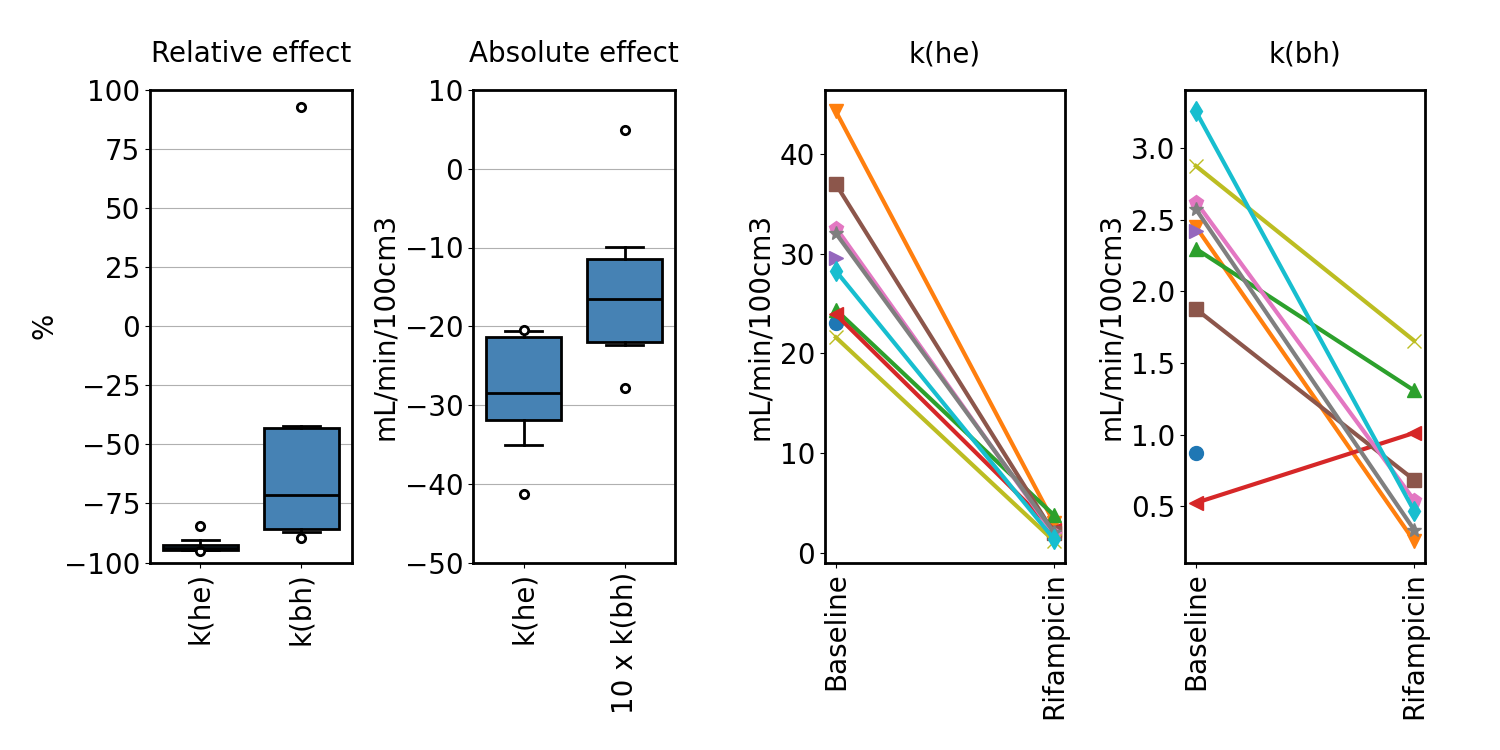
\includegraphics[width=6in]{C:/Users/md1spsx/Documents/GitHub/tristan-human-stage-3-analysis/build/Figs/fig_primary_outcomes.png}%
\caption{Visualisation of the primary endpoints khe and kbh across the population, showing a significant response to drug: (a) the relative and absolute effect size across the population as box plots; and (b) the individual values at control (left of plots) and after single dose of drug (right of plot). Colored lines in (b) represent individual volunteers. Note: absolute effect sizes for kbh have been scaled with a factor 10 to improve visualisation.}%
\end{figure}

%
\clearpage%


\begin{figure}[h!]%
\centering%
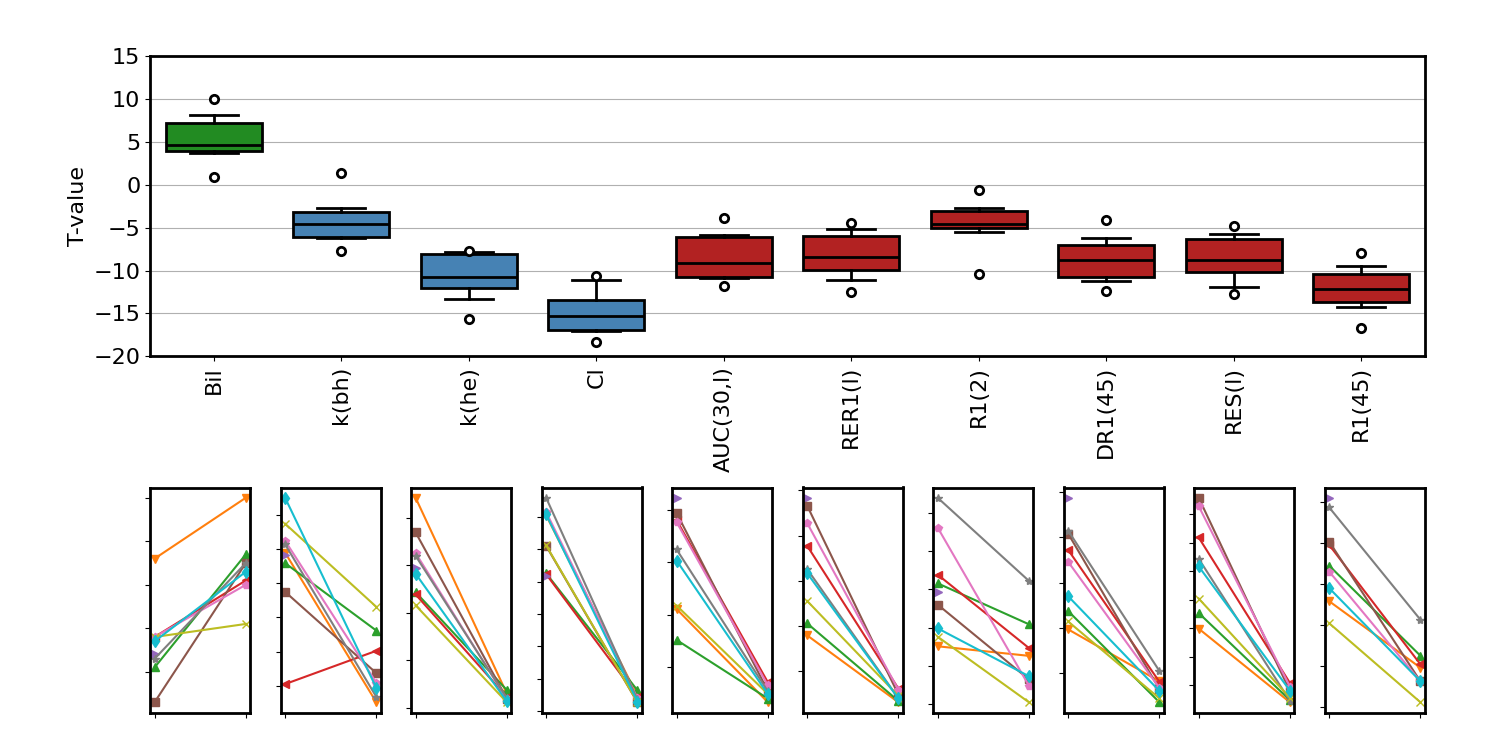
\includegraphics[width=6in]{C:/Users/md1spsx/Documents/GitHub/tristan-human-stage-3-analysis/build/Figs/fig_secondary_outcomes.png}%
\caption{drug effect for all parameters that show a significant reduction in the mean value (p<0.01). The top row shows the difference relative to the standard error of the difference, and the bottom row shows the individual effects for the corresponding biomarkers.}%
\end{figure}

%
\clearpage%


\begin{figure}[h!]%
\centering%
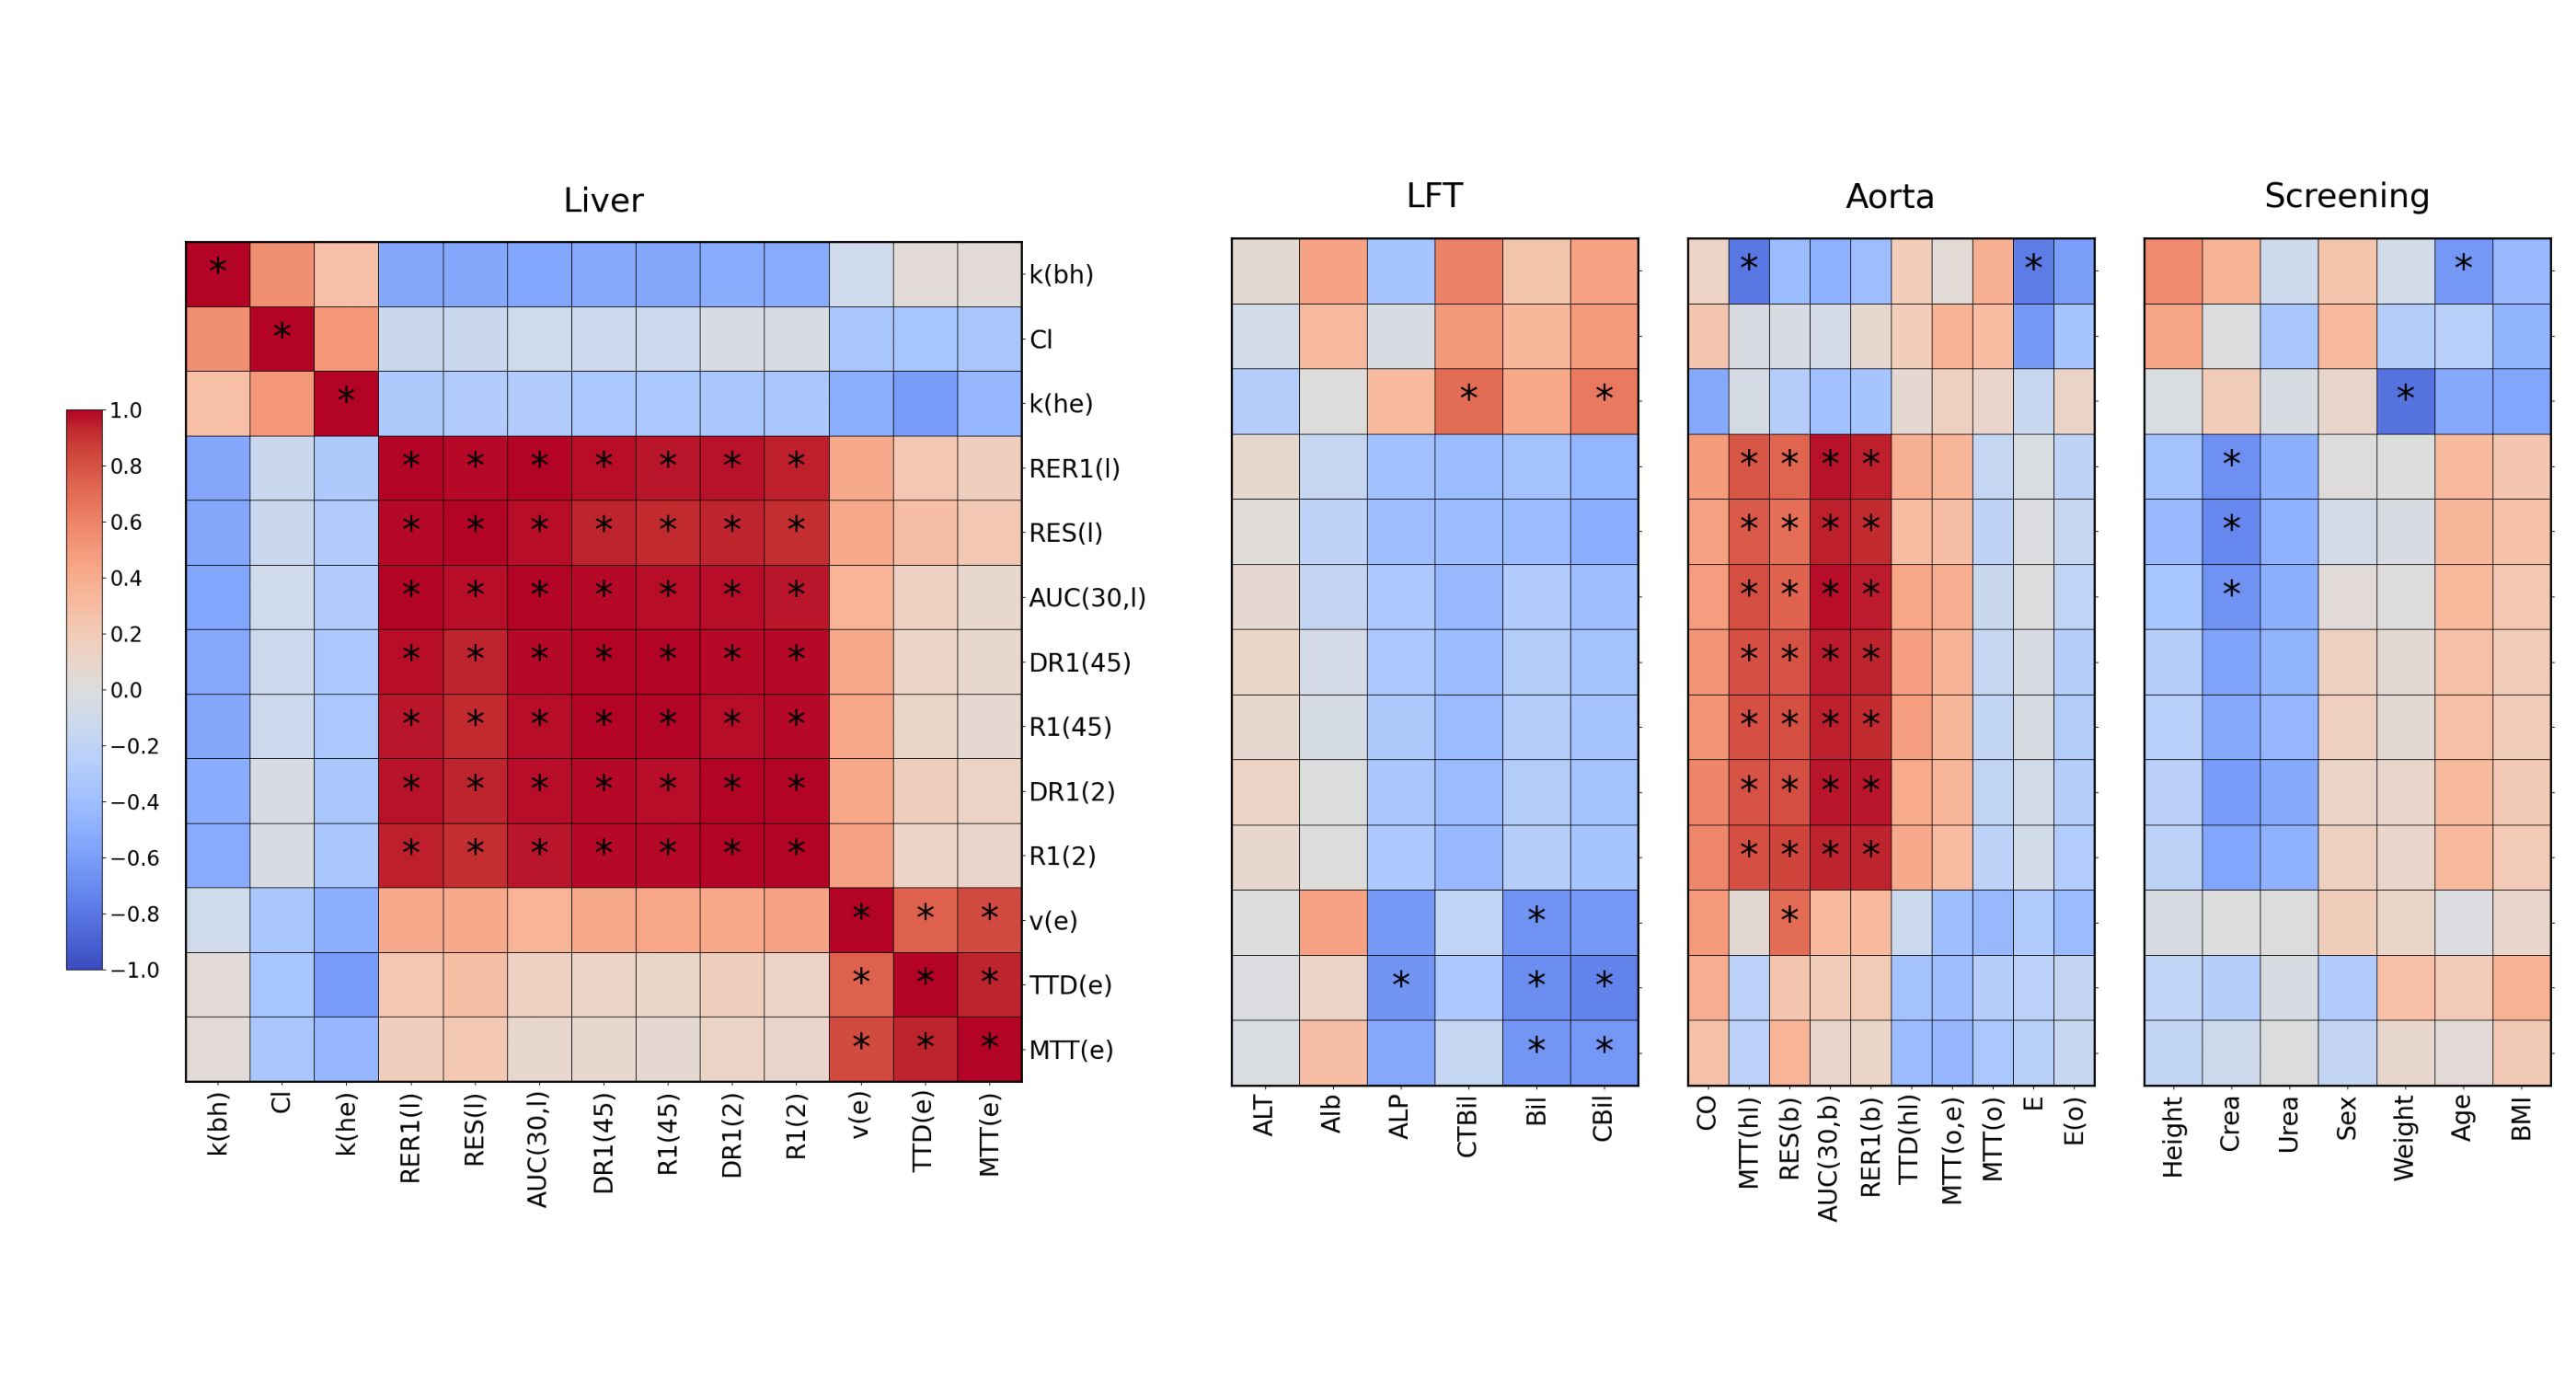
\includegraphics[width=6in]{C:/Users/md1spsx/Documents/GitHub/tristan-human-stage-3-analysis/build/Figs/fig_correlations_control.png}%
\caption{Correlations between parameters at control.}%
\end{figure}

%
\clearpage%


\begin{figure}[h!]%
\centering%
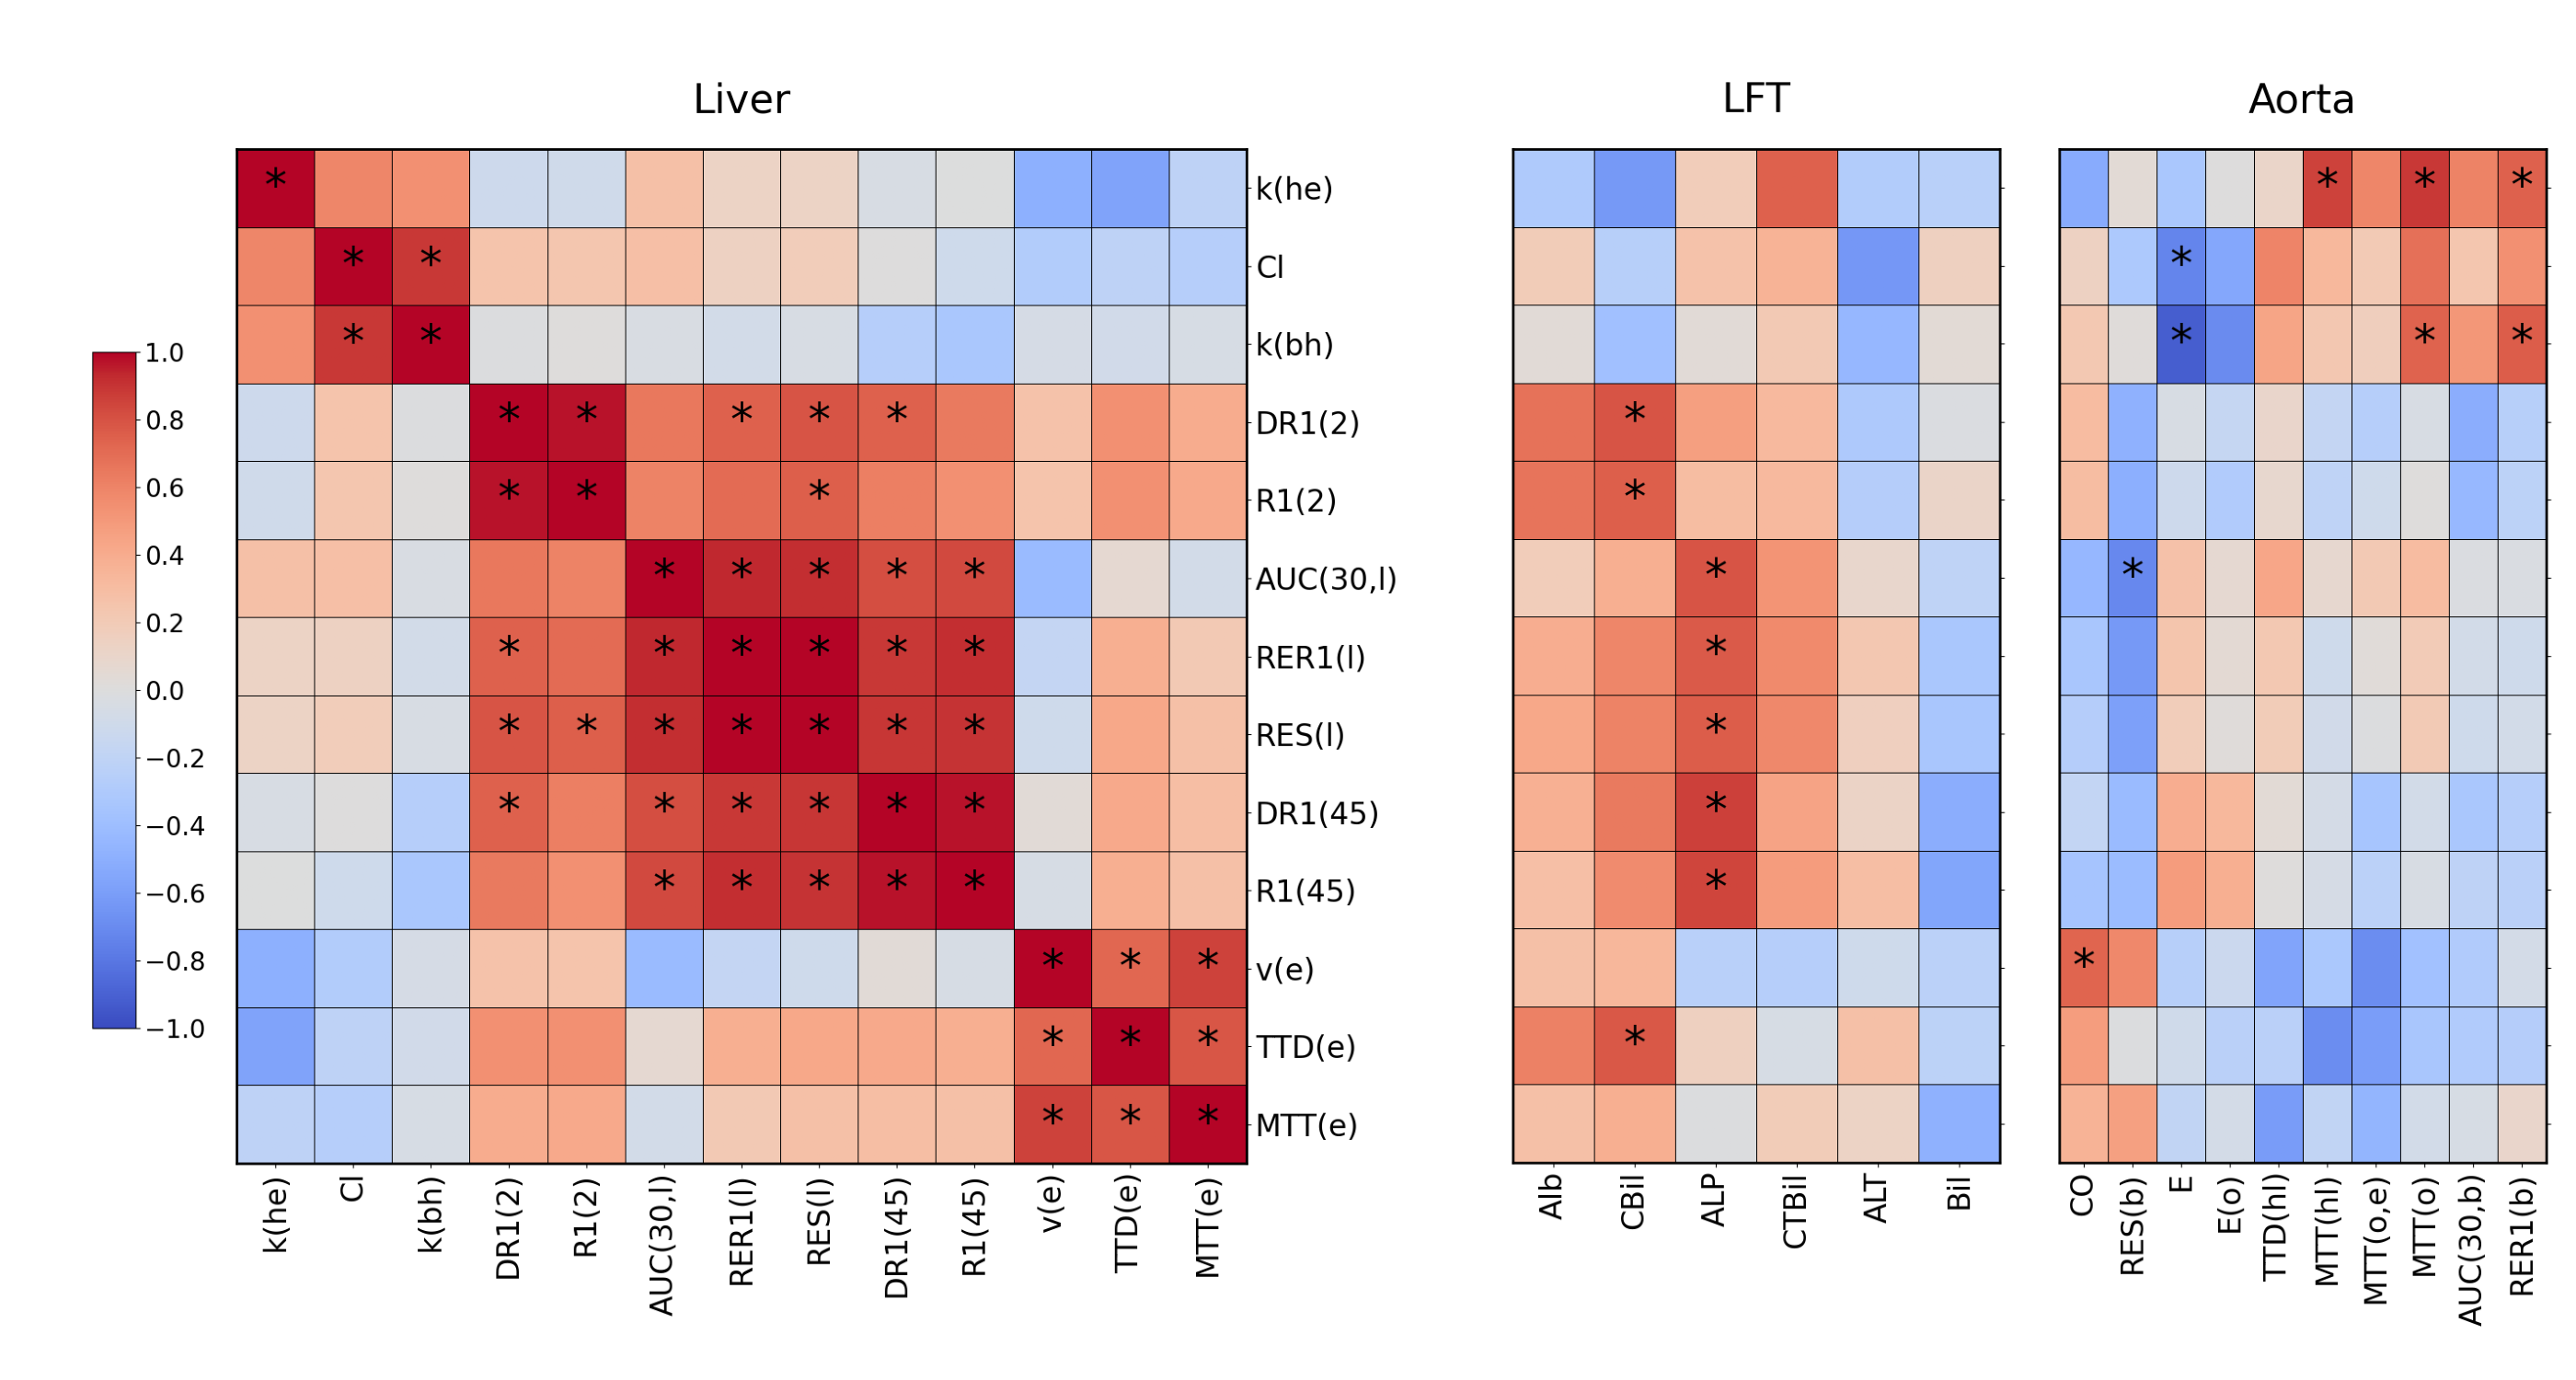
\includegraphics[width=6in]{C:/Users/md1spsx/Documents/GitHub/tristan-human-stage-3-analysis/build/Figs/fig_correlations.png}%
\caption{Correlations between parameter changes.}%
\end{figure}

%
\clearpage%
\chapter{Tables}%
\begin{longtable}{rcccccccc}%
\hline%
parameter&count&mean&std&min&25\%&50\%&75\%&max\\%
\hline%
Age (yr)&10.0&32.5&8.3&21.0&27.0&32.0&35.5&51.0\\%
ALP (U/L)&10.0&67.8&26.5&39.5&53.4&60.0&67.5&118.0\\%
ALT (U/L)&10.0&20.8&8.2&14.0&16.5&17.8&23.4&41.5\\%
Albumin (g/L)&10.0&42.3&2.8&37.0&41.8&42.8&43.4&46.0\\%
Bilirubin (umol/L)&10.0&13.0&4.2&6.5&10.8&12.8&14.0&23.0\\%
Conjugated Bilirubin (umol/L)&10.0&4.7&2.1&3.0&3.5&4.2&5.0&10.0\\%
Conjugated/total bilirubin (\%)&10.0&36.2&6.4&25.0&33.4&36.2&39.0&46.5\\%
BMI  (kg/m2)&10.0&24.4&3.5&18.7&22.6&24.0&26.8&30.0\\%
Creatinine (umol/L)&10.0&77.1&13.3&58.0&67.2&79.5&86.8&98.0\\%
Height  (cm)&10.0&174.3&8.1&163.1&167.6&175.7&179.9&187.8\\%
Urea nitrogen (mmol/L)&10.0&5.8&1.5&3.4&5.0&5.8&7.0&7.8\\%
Body weight  (kg)&10.0&73.2&7.6&57.0&72.8&74.6&75.9&82.8\\%
\hline%
\caption{Demographics of the study population.} \\%
\end{longtable}%
\clearpage%
\begin{longtable}{rcccc}%
\hline%
parameter&V1&V2&Diff&p\\%
\hline%
ALP&67.6 (40.1)&69.4 (54.1)&1.8 (23.1)&0.687\\%
ALT&21.8 (18.7)&25.4 (18.9)&3.6 (9.4)&0.069\\%
Alb&44.5 (4.1)&43.9 (5.9)&{-}0.6 (6.3)&0.598\\%
Bili&12.1 (8.5)&11.4 (9.3)&{-}0.8 (11.6)&0.731\\%
ConBili&4.8 (3.7)&4.6 (4.2)&{-}0.1 (5.1)&0.89\\%
ConTotBili&39.4 (11.3)&37.3 (9.1)&{-}3.0 (15.6)&0.358\\%
\hline%
\caption{LFT changes between both visits.} \\%
\end{longtable}%
\clearpage%
\begin{longtable}{|p{1.5cm}|p{1.5cm}|p{1.5cm}|p{1.5cm}|p{1.5cm}|p{1.5cm}|p{1.5cm}|}%
\hline%
Name&Group&control&drug&Effect size (\%)&T&p{-}value\\%
\hline%
Bilirubin (umol/L)&Blood {-} liver function test&13.0 (2.6) &22.0 (2.8) &81.9 (52.0) &{-}5.4&0.001\\%
Conjugated Bilirubin (umol/L)&Blood {-} liver function test&4.7 (1.3) &12.6 (6.2) &146.0 (57.0) &{-}3.1&0.02\\%
Albumin (g/L)&Blood {-} liver function test&42.3 (1.7) &40.9 (1.8) &{-}4.15 (2.9) &2.8&0.028\\%
Conjugated/total bilirubin (\%)&Blood {-} liver function test&36.2 (4.0) &44.6 (5.3) &23.1 (21.0) &{-}2.0&0.092\\%
ALT (U/L)&Blood {-} liver function test&20.8 (5.1) &24.1 (6.5) &17.4 (23.0) &{-}1.6&0.163\\%
ALP (U/L)&Blood {-} liver function test&67.8 (16.0) &73.9 (21.0) &{-}0.542 (11.0) &{-}0.0&0.986\\%
Liver blood clearance (L/min)&MRI {-} liver&0.265 (0.028) &0.0199 (0.0044) &{-}92.3 (2.5) &14.6&0.0\\%
R1 at 45mins (1/sec)&MRI {-} liver&2.33 (0.82) &1.38 (0.083) &{-}26.1 (3.2) &12.1&0.0\\%
Hepatocellular uptake rate (mL/min/100cm3)&MRI {-} liver&29.7 (4.5) &2.17 (0.59) &{-}92.6 (2.5) &10.6&0.0\\%
RE for Sl at 20min (\%)&MRI {-} liver&66.0 (23.0) &6.54 (1.7) &{-}87.5 (1.9) &8.8&0.0\\%
Delta R1 at 45mins (1/sec)&MRI {-} liver&1.07 (0.81) &0.136 (0.03) &{-}77.1 (5.8) &8.7&0.0\\%
AUC for Cl (0{-}35min) (mM*sec)&MRI {-} liver&205.0 (100.0) &25.8 (4.3) &{-}81.9 (2.7) &8.6&0.0\\%
RE for R1l at 20min (\%)&MRI {-} liver&86.9 (40.0) &8.86 (1.5) &{-}85.6 (1.9) &8.3&0.0\\%
R1 (scan 2) (1/sec)&MRI {-} liver&1.73 (0.44) &1.32 (0.071) &{-}11.7 (4.6) &4.5&0.003\\%
Biliary excretion rate (mL/min/100cm3)&MRI {-} liver&2.17 (0.54) &0.791 (0.34) &{-}48.7 (42.0) &4.1&0.005\\%
Delta R1 (scan 2) (1/sec)&MRI {-} liver&0.459 (0.43) &0.0757 (0.018) &{-}31.4 (76.0) &3.1&0.017\\%
Liver extracellular volume fraction (mL/100cm3)&MRI {-} liver&17.7 (6.5) &21.5 (3.3) &264.0 (420.0) &{-}1.4&0.199\\%
Extracellular mean transit time (sec)&MRI {-} liver&36.5 (11.0) &43.0 (7.7) &148.0 (240.0) &{-}0.9&0.406\\%
Extracellular dispersion (\%)&MRI {-} liver&66.1 (16.0) &70.4 (4.8) &283.0 (550.0) &{-}0.7&0.531\\%
\hline%
\caption{Univariate data analysis (liver).} \\%
\end{longtable}%
\clearpage%
\begin{longtable}{|p{1.5cm}|p{1.5cm}|p{1.5cm}|p{1.5cm}|p{1.5cm}|p{1.5cm}|p{1.5cm}|}%
\hline%
Name&Group&control&drug&Effect size (\%)&T&p{-}value\\%
\hline%
Organs extraction fraction (\%)&MRI {-} aorta&18.4 (3.2) &14.1 (3.2) &{-}25.4 (12.0) &4.0&0.005\\%
RE for R1b at 20min (\%)&MRI {-} aorta&20.6 (9.1) &22.9 (5.9) &45.2 (28.0) &{-}3.6&0.008\\%
AUC for Cb (0{-}35min) (mM*sec)&MRI {-} aorta&36.9 (16.0) &35.2 (8.1) &26.8 (16.0) &{-}3.5&0.011\\%
Body extraction fraction (\%)&MRI {-} aorta&6.73 (2.1) &3.46 (0.77) &{-}41.1 (16.0) &3.0&0.02\\%
Heart{-}lung dispersion (\%)&MRI {-} aorta&47.3 (8.7) &47.4 (8.0) &10.7 (9.8) &{-}2.0&0.087\\%
RE for Sb at 20min (\%)&MRI {-} aorta&15.3 (8.6) &20.2 (7.4) &136.0 (130.0) &{-}1.4&0.211\\%
Organs extravascular mean transit time (min)&MRI {-} aorta&5.98 (1.3) &6.72 (1.3) &31.4 (48.0) &{-}1.0&0.336\\%
Organs blood mean transit time (sec)&MRI {-} aorta&27.9 (5.5) &30.8 (7.0) &9.7 (20.0) &{-}0.8&0.464\\%
Heart{-}lung mean transit time (sec)&MRI {-} aorta&14.5 (3.3) &14.5 (2.5) &11.9 (23.0) &{-}0.7&0.514\\%
Cardiac output (L/min)&MRI {-} aorta&7.75 (2.0) &7.7 (1.2) &17.8 (27.0) &{-}0.6&0.54\\%
\hline%
\caption{Univariate data analysis (aorta).} \\%
\end{longtable}%
\clearpage%
\chapter{Supplements}%
\clearpage%


\begin{figure}[h!]%
\centering%
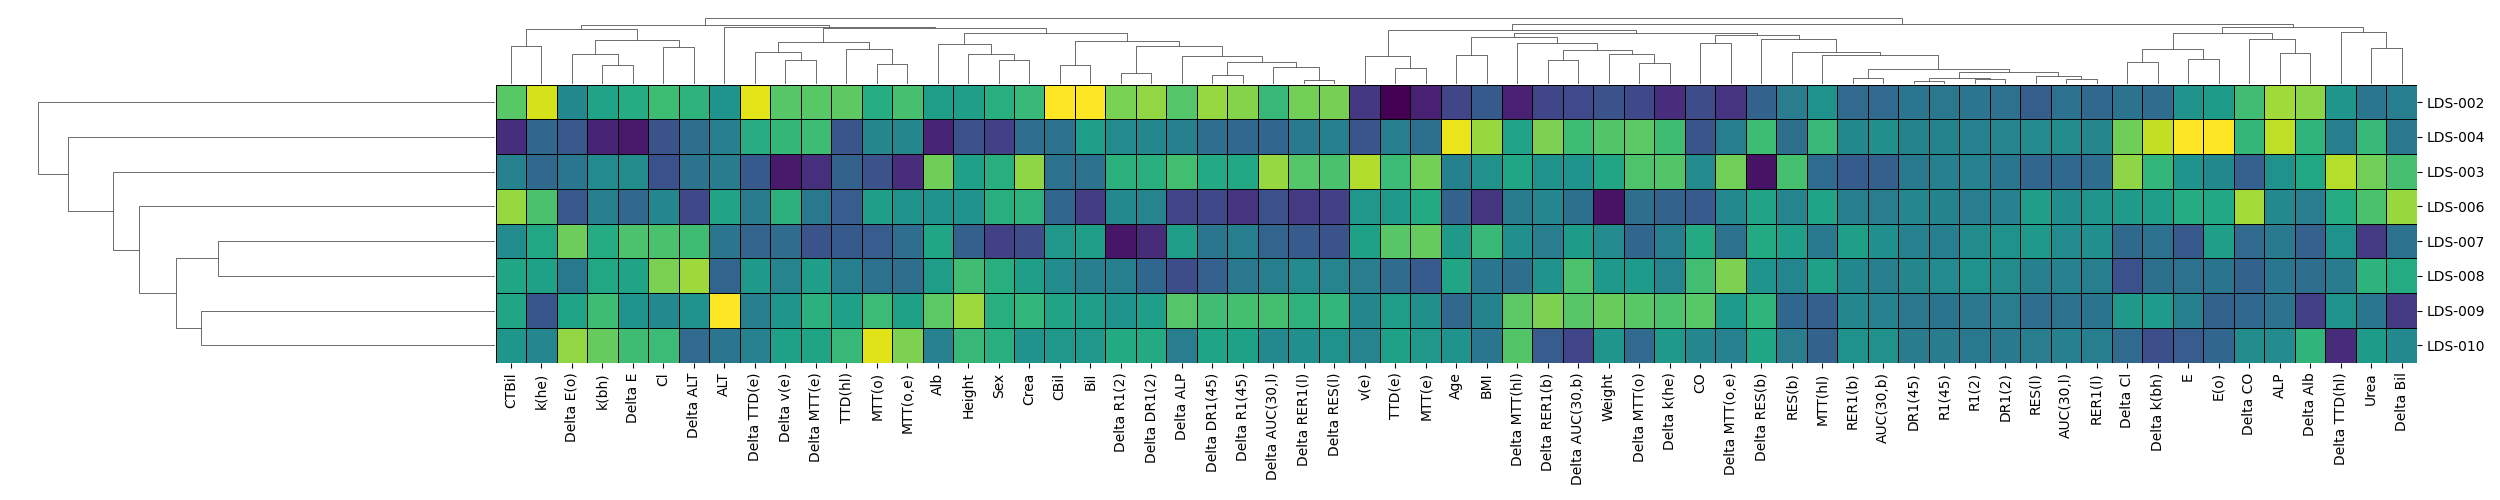
\includegraphics[width=6in]{C:/Users/md1spsx/Documents/GitHub/tristan-human-stage-3-analysis/build/Figs/fig_clustering.png}%
\caption{Clustering of parameters and subjects.}%
\end{figure}

%
\end{document}